\documentclass[conference]{IEEEtran}
\IEEEoverridecommandlockouts
% The preceding line is only needed to identify funding in the first footnote. If that is unneeded, please comment it out.
\usepackage{cite}
\usepackage{amsmath,amssymb,amsfonts}
\usepackage{algorithmic}
\usepackage{graphicx}
\usepackage{textcomp}
\usepackage{xcolor}
\usepackage[brazil]{babel}
\usepackage[utf8]{inputenc}
\usepackage{listings}
\usepackage{color}
\definecolor{codegreen}{rgb}{0,0.6,0}
\definecolor{codegray}{rgb}{0.5,0.5,0.5}
\definecolor{codedarkgray}{rgb}{0,0,0}
\definecolor{codeblue}{rgb}{0,0,1}
\definecolor{backcolour}{rgb}{0.95,0.95,0.92}
 \lstdefinestyle{mystyle}{
    backgroundcolor=\color{backcolour},   
    commentstyle=\color{codegreen},
    keywordstyle=\color{magenta},
    numberstyle=\tiny\color{codedarkgray},
    stringstyle=\color{codeblue},
    basicstyle=\footnotesize,
    breakatwhitespace=false,         
    breaklines=true,                 
    captionpos=b,                    
    keepspaces=true,                 
    numbers=left,                    
    numbersep=5pt,                  
    showspaces=false,                
    showstringspaces=false,
    showtabs=false,                  
    tabsize=2
}
 \lstset{style=mystyle}
\newcommand\tab[1][1cm]{\hspace*{#1}}
\usepackage{hyperref}
\def\BibTeX{{\rm B\kern-.05em{\sc i\kern-.025em b}\kern-.08em
    T\kern-.1667em\lower.7ex\hbox{E}\kern-.125emX}}

\title{Estudo e implementação de detecção de faces em imagens utilizando Python e a biblioteca DLIB}
\author{
    \IEEEauthorblockN{José B. M. Trineto \\ Werberson P. da Silva}
    \IEEEauthorblockA{
        \textit{Universidade de Brasília - Departamento de Engenharia Elétrica}
    }
}

\begin{document}
    \maketitle
    
    \begin{abstract}
        Redes neurais artificiais (ANNs do inglês \textit{Artificial Neural Networks}) tem sido a base para diversos modelos aplicados na área de visão computacional (CV do inglês \textit{Computer Vision}). Dentre as ANNs, podemos destacar as redes neurais convolucionais (CNNs do inglês \textit{Convolutional Neural Networks}) utilizadas para a construção de algoritmos de detecção de padrões em imagens. Neste artigo, será apresentado o estudo de CNNs aplicadas a CV e demonstrado o desenvolvimento de uma aplicação para o reconhecimento de faces humanas em imagens, utilizando a linguagem de programação Python em conjunto com a biblioteca DLIB. 
    \end{abstract}
    
    \begin{IEEEkeywords}
     	  Detecção Facial, Redes Neurais Convolucionais, Python, Biblioteca DLIB.
	 \end{IEEEkeywords}
	
    \section{INTRODUÇÃO}
		A detecção facial é uma técnica de CV utilizada para a detecção de faces humanas em imagens.	Apesar de ser um procedimento simples para os homens, é uma tarefa com um alto grau de complexidade para computadores, visto que rostos podem variar em iluminação, cor, posicionamento e escala. Existem uma gama de aplicações para a detecção facial, como exemplos, o reconhecimento de faces humanas, o autofoco utilizado em câmeras digitais, dentre outras.
		
	    As redes neurais convolucionais são utilizadas para a maioria das soluções de CV, aplicadas a uma ampla variedade de tarefas, dentre elas, a detecção facial. As CNNs tem apresentado resultados satisfatórios para problemas relacionados ao reconhecimento de padrões em imagens, com um custo computacional menor se comparado a uma rede neural clássica, pois buscam explorar subestruturas presentes nas imagens para otimizar o processamento.
	    
		Atualmente, diversas linguagens de programação e ferramentas possuem implementações que utilizam redes neurais convolucionais para a resolução de problemas relacionados a detecção de faces. Dentre estas soluções, podemos destacar a biblioteca DLIB utilizada em Python. Esta biblioteca foi escrita em C++ e permite a extração de 68 pontos na face, detectando o seu contorno, bem como o dos olhos, do nariz e da boca. Possui diversas vantagens em relação a outras implementações, tais como, o fácil aprendizado, a excelente documentação, a alta performance e etc Este artigo tem como objetivo a implementação de uma aplicação de em Python utilizando a biblioteca DLIB para a detecção de faces humanas em imagens.
		
		Este artigo está organizado da seguinte forma: a Seção II irá apresentar um estudo sobre os principais conceitos relacionados as redes neurais convolucionais no processamento de imagem; na Seção III será apresentado a aplicação desenvolvida em Python para o reconhecimento de faces humanas em imagens; a Seção IV mostrará os resultados obtidos da aplicação desenvolvida e a Seção V irá apresentar as conclusões.   
		
	 \section{REDES NEURAIS CONVOLUCIONAIS}
		As redes neurais convolucionais são redes neurais artificiais profundas que podem ser usadas para classificar imagens, extrair padrões e agrupá-las por similaridade, realizando o reconhecimento de objetos. São algoritmos que podem identificar rostos, objetos e outros aspectos dos dados visuais.

        CNNs apresentam uma camada de entrada e uma de saída e múltiplas camadas ocultas. As camadas ocultas são compostas por camadas convolucionais, de subamostragens (também conhecida como camada de \textit{pooling}) e por camadas completamente conectadas, como pode ser observado na Figura 1:
        
		\begin{figure}[h!b]
			\centering 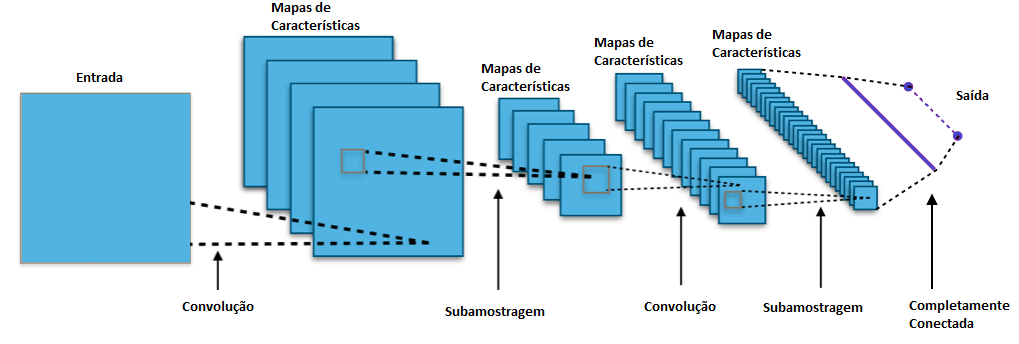
\includegraphics[width=10.5cm,height=5cm]{CNN}
			\caption{Exemplo de uma CNN com suas camadas (Baseado em \cite{b1})} 
		\end{figure}
		
		As camadas de convolução são responsáveis por identificar padrões e extrair diversas características da imagem, como bordas, cores e até mesmo padrões mais complexos de serem identificados, como olhos e narizes.  Esta camada é composta por um conjunto de filtros (ou \textit{kernels}) de convolução capazes de aprender de acordo com um treinamento. Os filtros são matrizes pequenas compostas por valores reais que podem ser interpretado como pesos. Esses filtros são convoluídos com os dados de entradas para obter um mapa de características. Estes mapas indicam regiões na qual padrões específicos em relação ao filtro, são encontradas na entrada. Os valores reais dos filtros se alteram ao longo do treinamento, do mesmo modo como os pesos de uma rede neural tradicional, fazendo com que a rede aprenda a identificar regiões significantes para extrair características do conjunto de dados.
		
		Um exemplo de convolução entre um filtro e uma imagem é apresentado na Figura 2:
		
		\begin{figure}[h!b]
			\centering 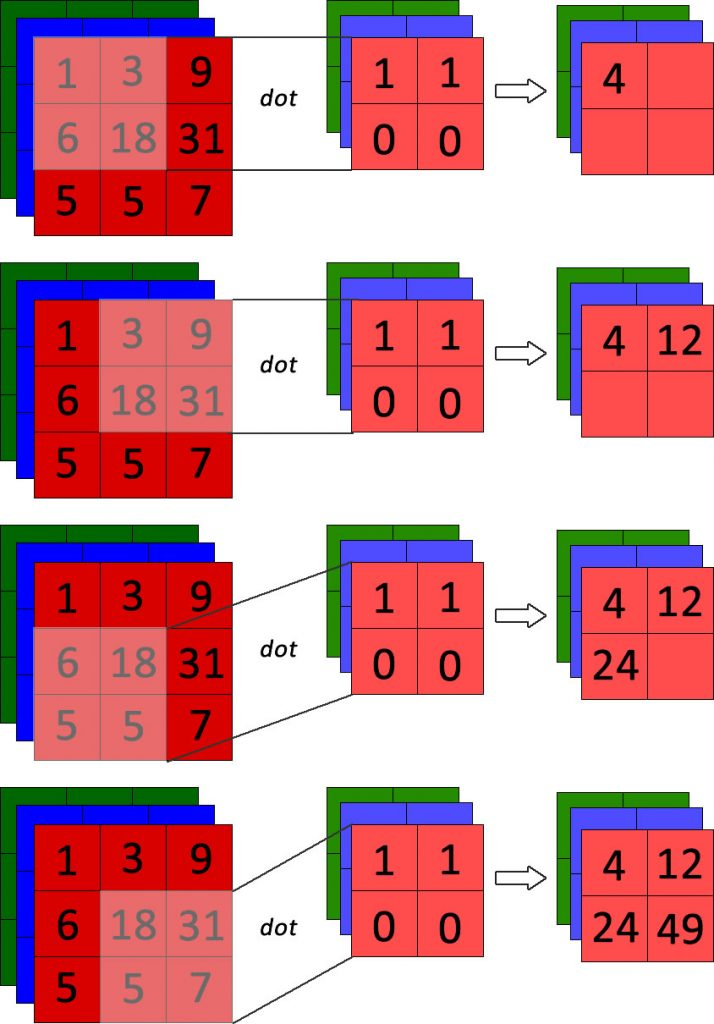
\includegraphics[width=5cm,height=6cm]{convolucao.jpg}
			\caption{Exemplo de convolução entre um filtro e uma imagem \cite{b2}} 
		\end{figure}
         
        Uma imagem é formada por um sistema de cores denominado RGB, em que o vermelho (\textit{red}), o verde (\textit{green}) e o azul (\textit{blue}) são combinados de várias formas de modo a reproduzir um largo espectro cromático. Neste exemplo, é apresentada uma imagem no sistema RGB 3 x 3 x 3 e um filtro 2 x 2 x 3. A convolução é realizada através do produto escalar de um pixel da imagem pelo filtro. Na sequência o filtro é deslizado para outra região e o produto escalar é realizado novamente até que toda a imagem seja percorrida. Cada canal é convoluído por uma dimensão diferente do filtro, que neste exemplo esta representado pela mesma cor do canal. O resultado final do processo de convolução é uma matriz chamada de mapa de características. Em cada camada de convolução de uma CNN pode ser aplicado o procedimento apresentado na Figura 2 para diferentes filtros, formando assim diversos mapas de características a cada camada convolutiva. 
        
         Após a operação de convolução apresentada na Figura 2, normalmente é aplicado uma função de ativação. Uma função bastante utilizada é a max(0,x), em que cada elemento menor do que zero, torna-se zero e os elementos maiores do que zero, permanecem com o mesmo valor.
         
         Traçando um paralelo com as RNAs, em uma camada convolutiva as entradas são os pixels da imagem e os pesos sinápticos são apresentados por cada valor contido no filtro. 

		  Após a camada de convolução, normalmente é utilizada uma camada de subamostragem. Esta camada tem por objetivo reduzir o tamanho espacial dos mapas de características gerados a partir do processo de convolução. Esta técnica reduz a quantidade de parâmetros a serem aprendidos na rede, diminuindo a complexidade da rede, desta maneira evitando o \textit{overfitting}. Algumas técnicas são aplicadas para a redução espacial das matrizes resultantes da convolução, como obtendo-se a soma, tirando a média, selecionando-se o maior (max \textit{pooling}) ou menor (min \textit{pooling}) da matriz em análise, desta maneira, produz-se uma sumarização do mapa de características. A Figura 3 apresenta um exemplo de utilização da técnica de max \textit{pooling}:
         
       \begin{figure}[h!b]
			\centering 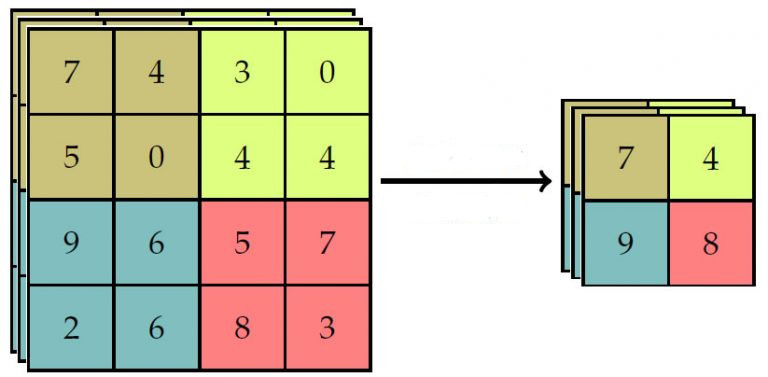
\includegraphics[width=5cm,height=2.7cm]{max-pooling.jpg}
			\caption{Exemplo de utilização da técnica de max \textit{pooling} \cite{b2}} 
		\end{figure}         
         
          A camada completamente conectada segue o mesmo princípio de uma rede neural multicamada tradicional em que cada camada é completamente conectada com a camada anterior.             
         
	 \section{APLICAÇÃO PARA DETECÇÃO DE FACES HUMANAS EM IMAGENS}
	 
          O programa abaixo foi utilizado para a detecção facial:	   
         
		  \begin{lstlisting}[breaklines=true, language=Python, caption=Programa utilizado para detecção facial]
import cv2
import dlib

imagem = cv2.imread("recursos/nome_imagem.extensao")
detector = dlib.cnn_face_detection_model_v1("recursos/mmod_human_face_detector.dat")
facesDetectadas = detector(imagem, 2)
for face in facesDetectadas:
    e, t, d, b = (int(face.rect.left()), int(face.rect.top()), int(face.rect.right()), int(face.rect.bottom()))
    cv2.rectangle(imagem, (e, t), (d, b), (255, 255, 0), 2)

cv2.imshow("Detector CNN", imagem)
cv2.waitKey(0)
cv2.destroyAllWindows()\end{lstlisting}


         Na linha 1 foi feito o \textit{import} da biblioteca openCV (cv2). Esta biblioteca será utilizada para ler a imagem, desenhar os retângulos das faces detectadas nas fotos e também por exibir a imagem com as faces detectadas. A documentação da openCV em python pode ser encontrada em \cite{b3}.
         
         Na linha 2 foi feito o \textit{import} da biblioteca DLIB. Esta biblioteca será utilizada para realizar a detecção de faces humanas em imagens utilizando uma rede neural convolucional. A documentação da DLIB em python pode ser encontrada em \cite{b4}.
         
         Na linha 4 foi feito o carregamento da imagem utilizando a função cv2.imread(). Na linha 5 o objeto dlib.cnn\_face\_detection\_model\_v1 detecta faces humanas em imagens. O construtor carrega o modelo de detecção facial de um arquivo. No código apresentado na \textit{Listing} 1, foi utilizado o modelo treinado disponível em \url{http://dlib.net/files/mmod\_human\_face\_detector.dat.bz2}. Este modelo é uma CNN que possui inicialmente 3 camadas de subamostragem, que terá por objetivo reduzir o tamanho da imagem em 8 vezes e tendo como saída um mapa de características com 32 dimensões. Logo após as camadas de subamostragens, existem mais 4 camadas de convolução. A plicação utilizada para construir a rede neural convolucional pode ser encontrada em \url{http://dlib.net/dnn\_mmod\_ex.cpp.html} O \textit{dataset} utilizado como treinamento para a CNN pode ser encontrado em \url{http://dlib.net/files/data/dlib_face_detection_dataset-2016-09-30.tar.gz}.
         
         Na linha 6, foi passados como argumento na função detector, a imagem carregada na linha 4 e o valor 2 como segundo argumento, que indica em quanto será aumentado a resolução da imagem. Quanto maior este argumento, maior será o número de faces detectadas na imagem e será exigido um maior poder de processamento da máquina que estiver rodando o programa. A função detector retorna as coordenadas das faces encontradas na imagem.
         
         As linhas 7, 8 e 9 são responsáveis por percorrer as coordenadas de todas as faces detectadas e desenhar um retângulo em volta de cada uma delas. Por fim, as linhas 11, 12 e 13 exibem a imagem com as faces detectadas.
         
         Foram utilizadas como entradas do programa apresentado na \textit{Listing} 1 as Figuras 4, 5 e 6:
         
         \begin{figure}[h!b]
			\centering 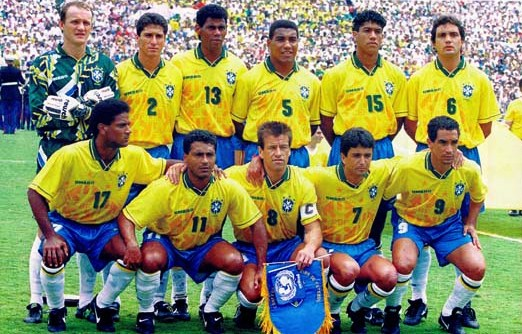
\includegraphics[width=7cm,height=3.7cm]{brasil_1994.jpg}
			\caption{Imagem utilizada como exemplo para detecção facial \cite{b5}} 
		\end{figure}
		
	    \begin{figure}[h!b]
			\centering 
\includegraphics[width=4cm,height=5.5cm]{matrix.jpg}
			\caption{Imagem utilizada como exemplo para detecção facial \cite{b6}} 
		\end{figure}

         \begin{figure}[h]
			\centering 
\includegraphics[width=7cm,height=3.7cm]{iron.jpg}
			\caption{Imagem utilizada como exemplo para detecção facial \cite{b7}} 
		\end{figure}

\bigskip
\bigskip
\bigskip

	\section{RESULTADOS OBTIDOS}
        Como podem ser visto nas Figuras 4, 5 e 6, foram utilizadas imagens com características diferentes. A Figura 4 (522 x 334 pixels), foto da seleção brasileira de 1994, é uma imagem que não possui uma boa qualidade, em que existem 11 faces humanas masculinas com cores de peles diferentes. A Figura 5 (330 x 488 pixels), foto do pôster do filme Matrix, existem 3 faces humanas masculina e 1 feminina e possui tom de cores voltados para o preto e o branco . Todas as faces estão utilizando óculos escuros e duas são carecas. A imagem 6 (699 x 420), foto de um show da banda de rock Iron Maiden, possui 3 faces humanas masculinas, em que duas delas possuem cabelos grandes e outra está com com um microfone próxima a boca. Nesta foto, cada face possui uma inclinação diferentes. 
        
        
		As Figuras 7, 8 e 9 são as saídas do programa:
		
		 \begin{figure}[h!b]
			\centering 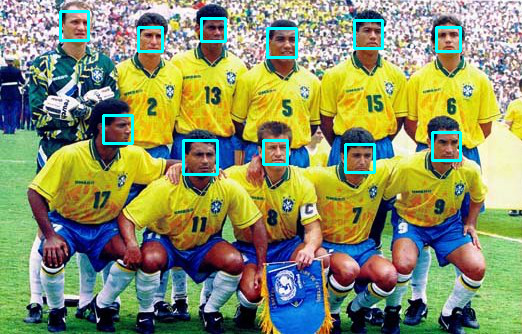
\includegraphics[width=7cm,height=3.7cm]{brasil_1994_detectada.png}
			\caption{Figura 4 com as faces detectadas} 
		\end{figure}
		
	    \begin{figure}[h!b]
			\centering 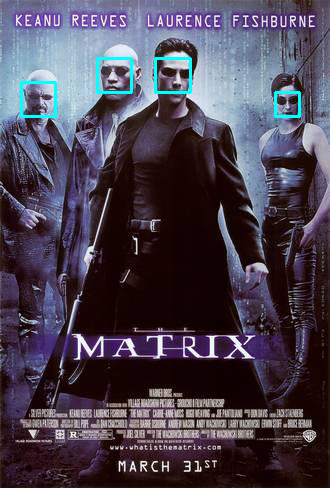
\includegraphics[width=4cm,height=5.5cm]{matrix_detectada.png}
			\caption{Figura 5 com as faces detectadas} 
		\end{figure}

         \begin{figure}[h]
			\centering 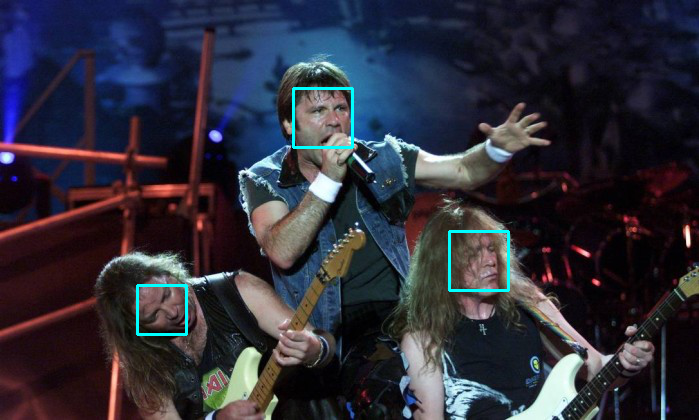
\includegraphics[width=7cm,height=3.7cm]{iron_detectada.png}
			\caption{Figura 6 com as faces detectadas} 
		\end{figure}
	
        Como podem ser visto nas Figuras 7, 8 e 9, todas as faces contidas nas três figuras foram identificadas. Uma métrica útil é a confiança que pode ser obtida com o uso da DLIB. Para isto, basta acessar o atributo confidence da classe dlib.mmod\_rectangle, isto pode ser feito com a substituição da linha 8 do programa apresentado na \textit{Listing} 1 pela seguinte linha apresentada na \textit{Listing 2}:
        
		\begin{lstlisting}[breaklines=true, language=Python, caption=Código para descobrir a confiança no DLIB]
    e, t, d, b, conf = (int(face.rect.left()), int(face.rect.top()), int(face.rect.right()), int(face.rect.bottom()), face.confidence)\end{lstlisting}

        Na \textit{Listing 2} foi adicionado a variável "conf" que irá receber o valor do atributo "face.confidence". Quanto maior o valor deste atributo, maior será a "certeza" de detecção de uma face humana. A Tabela 1 apresenta os níveis de confiança das faces detectadas para as três imagens:
        
		\begin{table}[h!b]
		\caption{valores de Confiança}
		\label{table}
		\setlength{\tabcolsep}{4pt}
		\begin{tabular}{|p{30pt}|p{50pt}|p{90pt}|p{50pt}|}
			\hline
				Figura & Número de faces detectadas & Valores de Confiança & Média dos valores de Confiança\\
			\hline
				Figura 7 & 11 & 1.0981, 1.0935, 1.0777, 1.0762, 1.0748, 1.0693, 1.0571, 1.0301, 0.9989, 0.9965, 0.9505 				& 1.0475 \\
			\hline
				Figura 8 & 4 & 1.0564, 1.0556, 1.0530, 1.0426 & 1.0512\\ 
			\hline
				Figura 9 & 3 & 1.1002, 0.9175, 0.8070 & 0.9416\\ 
			\hline
		\end{tabular}
		\label{tab1}
		\end{table}        
          
          A partir da Tabela 1 pode-se observar que as Figuras 7 e 8 apresentaram níveis médios de confiança próximos, sendo que a Figura 8 apresentou um valor ligeiramente maior. Por outro lado, a Figura 9 foi a que apresentou o menor valor dentre todas as imagens, isto pode ter ocorrido devido as faces na Figura 9 apresentarem uma maior inclinação e rotação se comparado as faces nas outras imagens.
	
	\section{CONCLUSÕES}
         Este artigo apresentou uma simples e eficiente aplicação escrita em Python para o reconhecimento de faces humanas em imagens baseado em um modelo que utiliza redes neurais convolucionais. Foram avaliadas 3 imagens com características diferentes, como qualidade, tons e faces com as mais variadas características. Nos 3 casos, a aplicação reconheceu todas as faces, apresentando excelentes resultados. 
        
         Apesar dos bons resultados obtidos com as imagens testadas, é recomendado o uso da biblioteca DLIB em máquinas que possuem um alto poder de processamento para o reconhecimento de faces em certas imagens.
      
         
	  \begin{thebibliography}{00}

		\bibitem{b1} https://en.wikipedia.org/wiki/Convolutional\_neural\_network, acessado em 24/06/2018	  
	  		
		\bibitem{b2} http://www.computacaointeligente.com.br/artigos/redes-neurais-convolutivas-cnn/, acessado em 		        21/06/2018.
		
		\bibitem{b3} https://docs.opencv.org//3.0-beta/doc/py\_tutorials/py\_tutorials.html, acessado em 24/06/2018.
		
		\bibitem{b4} http://dlib.net/python/index.html, acessado em 24/06/2018.
		
		\bibitem{b5} https://www.imortaisdofutebol.com/2012/12/19/selecoes-imortais-brasil-1994/, acessado em                                                                   		24/06/2018
		
		\bibitem{b6} http://www.allposters.com.br/-sp/Matrix-posters\_i8032466\_.html, acessado em 24/06/2018.

		\bibitem{b7} https://oglobo.globo.com/cultura/musica/iron-maiden-vem-ao-brasil-para-cinco-shows-em-						marco-17699861, acessado em 24/06/2018.
		
		\bibitem{b8} KING, Davis E. Dlib-ml: A machine learning toolkit. Journal of Machine Learning Research, v. 10, 			n. Jul, p. 1755-1758, 2009.
		
		\bibitem{b9} PROTAS, Églen da Veiga. Visualização de Camadas Intermediárias de Redes Neurais
		Convolucionais de Transformação de Imagem. 2017. 148 f. Dissertação (Mestrado) –
		Programa de Pós-Graduação em Computação. Universidade Federal do Rio Grande, Rio
		Grande.
		
		\bibitem{b10} Haykin, Simon S., et al. Neural networks and learning machines. Vol. 3. Upper Saddle River, NJ, 			USA:: Pearson, 2009.
		
	  \end{thebibliography}

\end{document}
